\section{Approach}

\begin{frame}
	\frametitle{Approach}
	\begin{columns}
		\begin{column}{0.6\textwidth}
			\begin{enumerate}
				\item Compiling Matlab code into intermediate representation
				\item Apply optimizations indenpendently of runtime specific system
				\item Compiling intermediate representation into runtime specific format
			\end{enumerate}
		\end{column}
		\begin{column}{0.4\textwidth}
			
\includegraphics[width=0.8\textwidth]{images/approach.jpg}
		\end{column}
	\end{columns}
\end{frame}

\begin{frame}
	\frametitle{System architecture}
	\begin{center}
		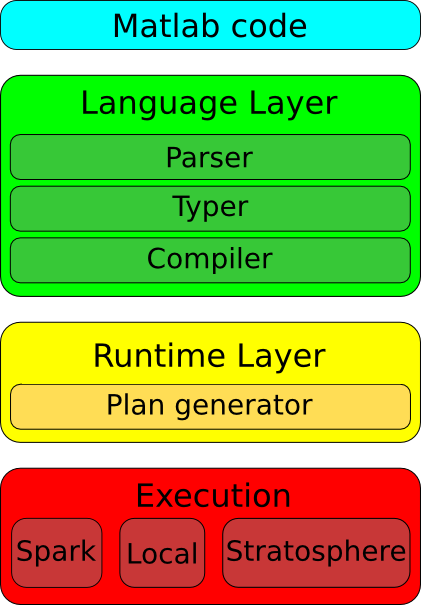
\includegraphics[height=0.8\textheight]{images/architecture.png}
	\end{center}
\end{frame}

\begin{frame}[fragile]
	\frametitle{Language}
	\begin{columns}
		\begin{column}{0.65\textwidth}
			\begin{itemize}
				\item Matlab-like language
				\item Support of basic linear algebra operations
				\item Some built-in functions, repmat, linspace, pdist2
				\item Loop support with static and dynamic termination criterion
				\item Language expressive enough to support variety of algorithms, Pagerank, K-means, NNMF
			\end{itemize}
		\end{column}
		\begin{column}{0.35\textwidth}
			\begin{lstlisting}[basicstyle=\scriptsize]
A'*B

f=@(x) x.^2.0

eps = 0.1

c=@(p,c) norm(p-c,2) < eps

fixpoint(1/2, f, 10, c)
			\end{lstlisting}
		\end{column}
	\end{columns}
\end{frame}

\begin{frame}
	\frametitle{Compilation: Intermediate format}
	\begin{itemize}
		\item Scala's combinator parsing tool box
		\item Powerful enough for our language
		\item Matlab is dynamically typed
		\item Execution on Stratosphere requires type knowledge at compilation time
		\item Hindley-Milner type inference algorithm to infer types and dimensions
	\end{itemize}
\end{frame}

\begin{frame}[fragile]
	\frametitle{Example: Parsing and typing}
	\begin{block}{Input}
\begin{lstlisting}[language=Matlab]
A = ones(2,10);
B = eye(10,3);
A*B
\end{lstlisting}
\end{block}
	
\begin{block}{Parsed and typed}	
\begin{lstlisting}[language=Matlab]
A = ones(2,10):MatrixType[Double,2,10];
B = eye(10,3):MatrixType[Double,10,3];
A*B:MatrixType[Double,2,3]
\end{lstlisting}
\end{block}

\end{frame}

\begin{frame}[fragile]
	\frametitle{Example: Intermediate code}
	\begin{block}{Compiled}
\begin{lstlisting}[columns=flexible, language=Java]
MatrixMult(
  ones(
    IntValue(2),
    IntValue(10)
  ), 
  eye(
    IntValue(10),
    IntValue(3)
  )
)
\end{lstlisting}
	\end{block}
\end{frame}

\begin{frame}
	\frametitle{Example: Stratosphere execution plan}
	\begin{center}
		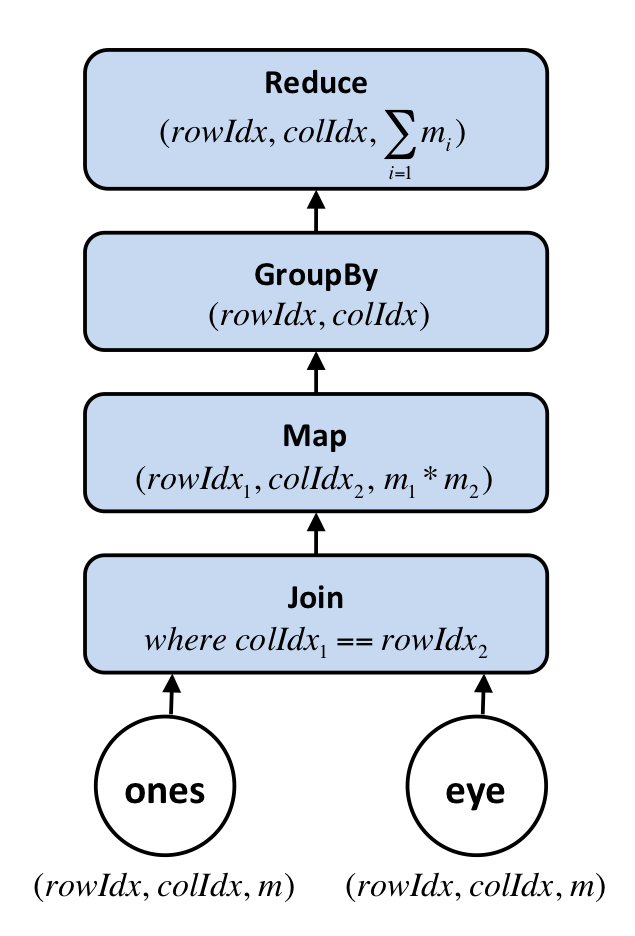
\includegraphics[height=0.9\textheight]{images/matrixMultDataflow.png}
	\end{center}
\end{frame}